
\documentclass{beamer}
\setbeamercolor{frametitle}{fg=white}
\setbeamercolor{title}{fg=white}
\setbeamercolor{author}{fg=white}
\setbeamercolor{date}{fg=white}
\setbeamercolor{normal text}{fg=white}

\usetheme{default}
\usepackage{graphicx}

\setbeamertemplate{background canvas}{%

\includegraphics[width=\paperwidth,height=\paperheight]{./images/background.png}}

\title{Predstavitev:\\Avtomatizirano Ustvarjanje Prosojnic z AI}
\author{Ime Avtorja\\[1ex]{\small Afiliacija Avtorja}}
\date{\today}

\begin{document}

\begin{frame}
\titlepage
\centering
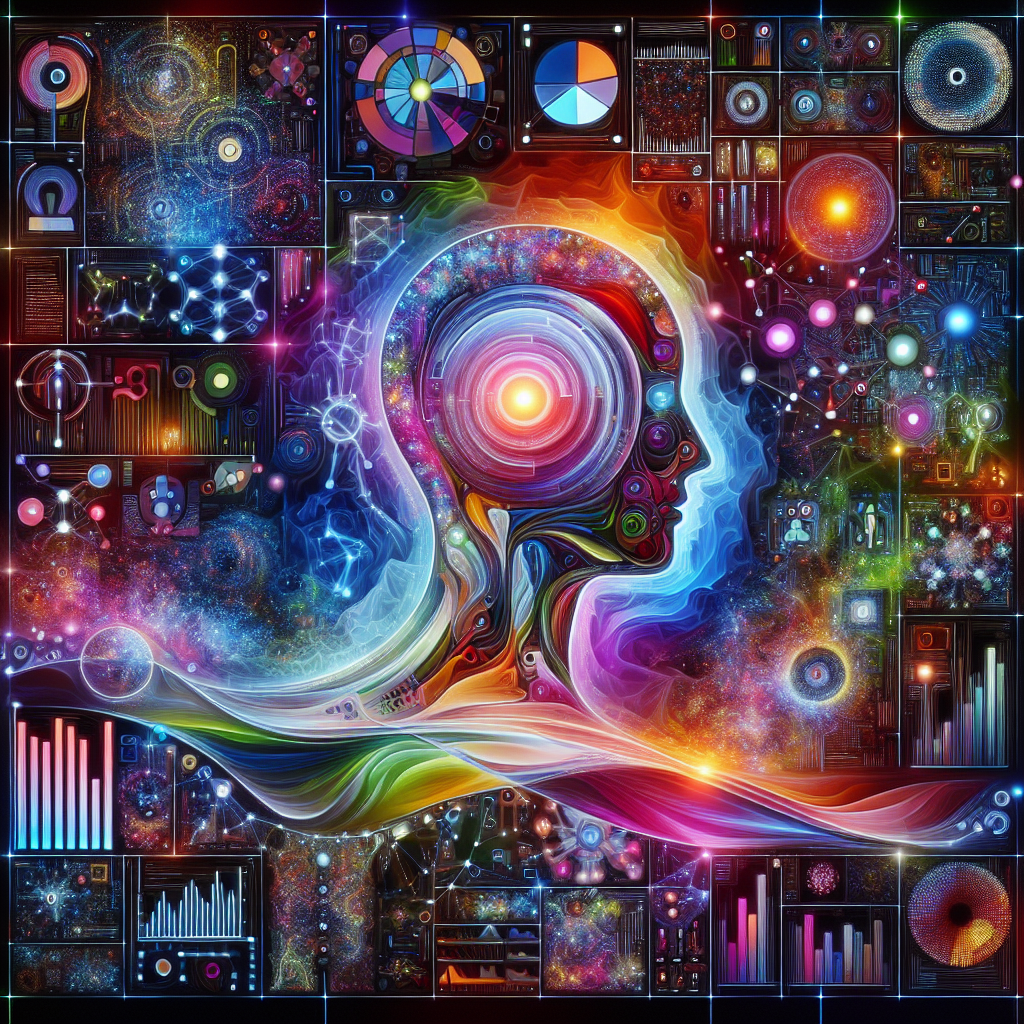
\includegraphics[width=0.5\textwidth]{./images/title_image.png}
\end{frame}

\begin{frame}{Uvod}
\begin{itemize}
    \item Pozdravljamo vas pri predstavitvi revolucionarne AI re�itve.
    \item AI program poenostavlja proces ustvarjanja prosojnic za vsakogar.
    \item Vnesite temo, skript ali seminarsko nalogo, in program ustvari prosojnice.
\end{itemize}
\centering

\includegraphics[width=0.5\textwidth]{./images/introduction.png}
\end{frame}

\begin{frame}{Kako deluje?}
\begin{itemize}
    \item Delovanje preko enostavnih API klicev.
    \item Vnos teme, skripta ali nalogo v program.
    \item AI analizira vsebino, strukturira informacije in ustvari prosojnice.
    \item Mo�nost prilagoditve rezultatov, da popolnoma ustrezajo va�im potrebam.
\end{itemize}
\centering
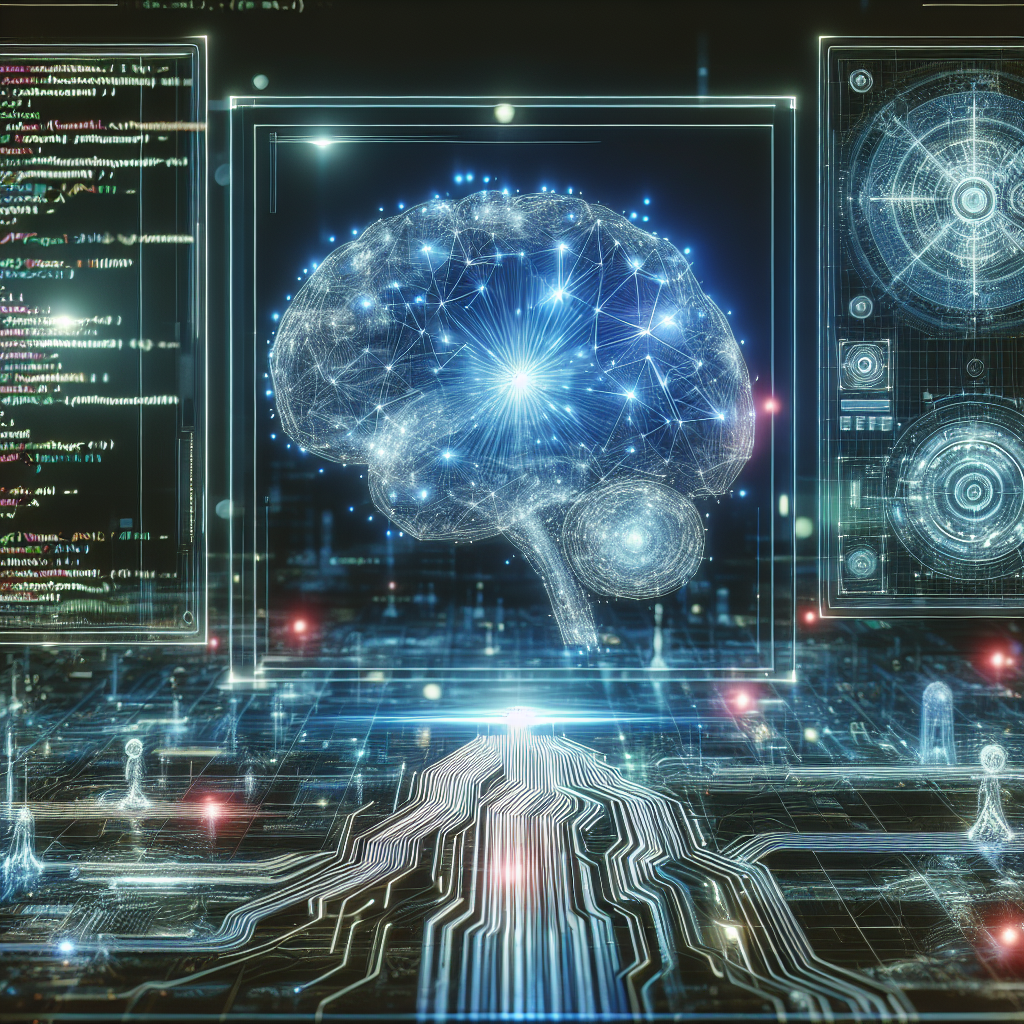
\includegraphics[width=0.5\textwidth]{./images/how_it_works.png}
\end{frame}

\begin{frame}{Prednosti}
\begin{itemize}
    \item Prihranek asa: avtomatizacija ustvarjanja prosojnic.
    \item Manj truda: zmanj�ano rono delo pri oblikovanju prosojnic.
    \item Fleksibilnost: prilagodljivost rezultatov glede na va�e zahteve.
    \item Iterativni proces: mo�nost izbolj�anja rezultatov z vnasanjem povratnih informacij.
\end{itemize}
\centering
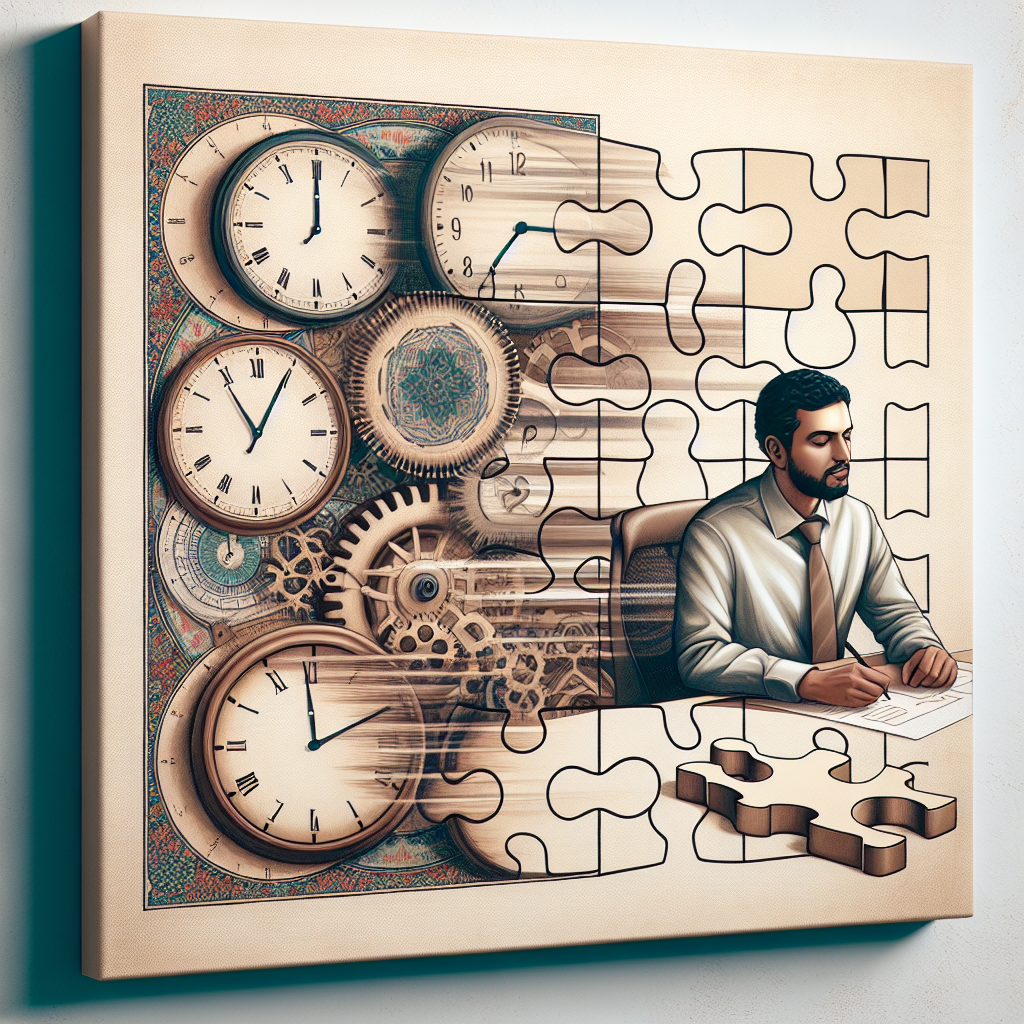
\includegraphics[width=0.5\textwidth]{./images/benefits.png}
\end{frame}

\begin{frame}{Primeri Uporabe}
\begin{itemize}
    \item �tudentske predstavitve.
    \item Poslovne in marketin�ke predstavitve.
    \item Uitelji, ki pripravljajo une materiale.
    \item Vsak, ki potrebuje hitro, a profesionalno ustvarjene prosojnice.
\end{itemize}
\centering

\includegraphics[width=0.5\textwidth]{./images/use_cases.png}
\end{frame}

\begin{frame}{Zakljuek}
\begin{itemize}
    \item Na� AI program prina�a inovativno re�itev v svet predstavitev.
    \item Preprosta uporaba, visoka prilagodljivost in uinkovitost.
    \item Preizkusite danes in izbolj�ajte va�e predstavitve z minimalnim trudom!
\end{itemize}
\centering

\includegraphics[width=0.5\textwidth]{./images/conclusion.png}
\end{frame}

\begin{frame}{Vpra�anja?}
\centering

\includegraphics[width=0.5\textwidth]{./images/questions.png}
\end{frame}

\begin{frame}{Hvala za pozornost!}
\centering

\includegraphics[width=0.5\textwidth]{./images/thank_you.png}
\end{frame}

\end{document}
